Chirp-pulsed amplification and the effects of phase delay in a Michelson interferometer.
\begin{parts}
	\part Phase acquired by a pulse in a dispersive medium of length $z$ (assuming homogeneity):
	\begin{align*}
		\phi(\omega) &= k(\omega) \cdot z \\
		&= \phi(\omega_0) + \phi^{(1)}(\omega_0) \cdot (\omega - \omega_0) + \frac{1}{2} \phi^{(2)}(\omega_0) \cdot (\omega - \omega_0)^2 + \ldots
	\end{align*}
	by Taylor expanding around the carrier frequency $\omega_0$.
	
	Here group delay is:
	\begin{align*}
		\phi^{(1)} &= \evalat{\deri{\phi}{\omega}}{\omega_0} \\
		&= \evalat{\deri{k}{\omega}}{\omega_0} \cdot z \\
		&= \frac{z}{v_g (\omega_0)} \mtext{where $v_g = \dderi{\omega}{k}$ is group velocity}
	\end{align*}
	
	Group delay dispersion (GDD):
	\begin{align*}
		\phi^{(2)} &= \evalat{\deri[2]{\phi}{\omega}}{\omega_0} \\
		&= \evalat{\diff{\omega} \rbracket{\frac{z}{v_g}}}{\omega_0} \\
		&= \evalat{\deri{v_g^{-1}}{\omega}}{\omega_0} \cdot z
	\end{align*}
	
	Now consider the time taken for a spectral component of frequency $\omega$ to pass through the medium:
	\begin{gather*}
		\phi(\omega) = \indefint{T(\omega)}{\omega} \\
		\Rightarrow T(\omega) = \pderi{\phi}{\omega} \\
		= T(\omega_0) + \evalat{\pderi{T}{\omega}}{\omega_0} (\omega - \omega_0) + \ldots \mtext{by Taylor expansion} \\
		= \phi^{(1)} + \phi^{(2)} \cdot (\omega - \omega_0) + \ldots
	\end{gather*}
	
%	So for an input E field $E_\textnormal{in}(t) = \diagfrac{1}{\sqrt{2\pi}} \int_{-\infty}^{\infty} a(\omega) \mathrm{e}^{-i\omega t} \mathrm{d}\omega$, we have output:
%	\begin{align*}
%		E_\textnormal{out}(t) &= \frac{1}{\sqrt{2\pi}} \int_{-\infty}^{\infty} a(\omega) \mathrm{e}^{i\phi(\omega)} \mathrm{e}^{-i\omega t}\,\mathrm{d}\omega \\
%		&= \frac{1}{\sqrt{2\pi}} \cdot \mathrm{e}^{i\sbracket{\phi(\omega_0) - \phi^{(1)}\cdot\omega_0}} \int_{-\infty}^{\infty} a(\omega) \mathrm{e}^{-i\sbracket{\omega t - \phi^{(1)}\omega}}\,\mathrm{d}\omega \mtext{ignoring higher order terms} \\
%		&= \frac{1}{\sqrt{2\pi}}
%		{\color{green}
%			\underbracket{\color{black} \mathrm{e}^{i\sbracket{k(\omega_0)z - \omega_0 T(\omega_0)}}}_{\color{black}\textnormal{carrier wave}}
%		}
%		{\color{blue}
%			\underbracket{\color{black} \int_{-\infty}^{\infty} a(\omega) \mathrm{e}^{-i\omega\sbracket{t - z/v_g}}\,\mathrm{d}\omega}_{\color{black}\textnormal{envelope}}
%		}
%	\end{align*}
%	
%	Note that the {\color{green}carrier wave} travels at a different velocity than the {\color{blue}envelope}:
	
%	$\color{green} v_p = \dfrac{\omega_0}{k(\omega_0)}$ is phase velocity and $\color{blue} v_g$ is the group velocity.
	
	\newpage
	In general phase velocity $v_p = \dfrac{\omega_0}{k(\omega_0)} \neq v_g$, so what $\phi^{(1)}$ is responsible for is introducing the carrier-envelope offset (CEO) where the peak of a pulse drifts away from the envelope peak.
	\begin{figure}[H]
		\centering
		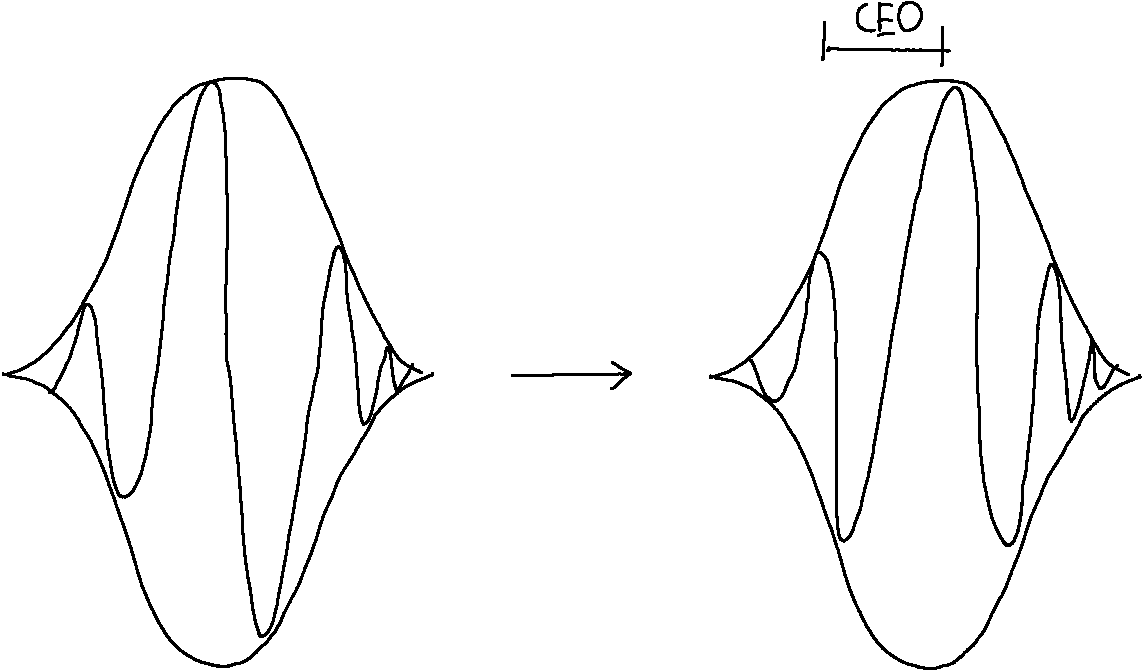
\includegraphics[width=.9\linewidth]{q1-ceo}
	\end{figure}
	
	As for $\phi^{(2)}$, note that it has a linear contribution to $T(\omega) \Rightarrow \phi^{(2)}$ separates each frequency component and distorts the pulse, e.g. for $\phi^{(2)} > 0$ we have positive chirp where higher frequencies are pushed towards the back of a pulse.
	\begin{figure}[H]
		\centering
		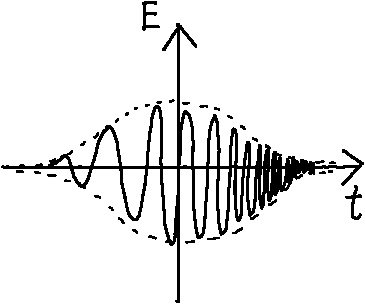
\includegraphics[width=.4\linewidth]{q1-cpa}
	\end{figure}
	
	Ultrashort laser pulses are typically generated by modelocked lasers, which usually possess low energy ($\sim \unit{\nano\joule}$).
	However, owing to its short pulse duration, simple amplification would lead to extremely large peak intensities.
	
	Multiple complications arise as a results:
	\begin{enumerate}
		\item First we have self-modulation of the pulse due to the large B-integral.
		This leads to complicated phase structure that is difficult to undo.
		
		\item We also have self-focusing that leads to regions of intensities so great that the optical elements may be damaged.
	\end{enumerate}
	
	To counter this, chirped-pulse amplification (CPA) is used instead to stretch the input pulse before amplification, thereby avoiding large peak intensities.
	The amplified pulse is then compressed before output, leading to high power ultrashort laser pulse.
	
	Schematic of a CPA system:
	\begin{figure}[H]
		\centering
		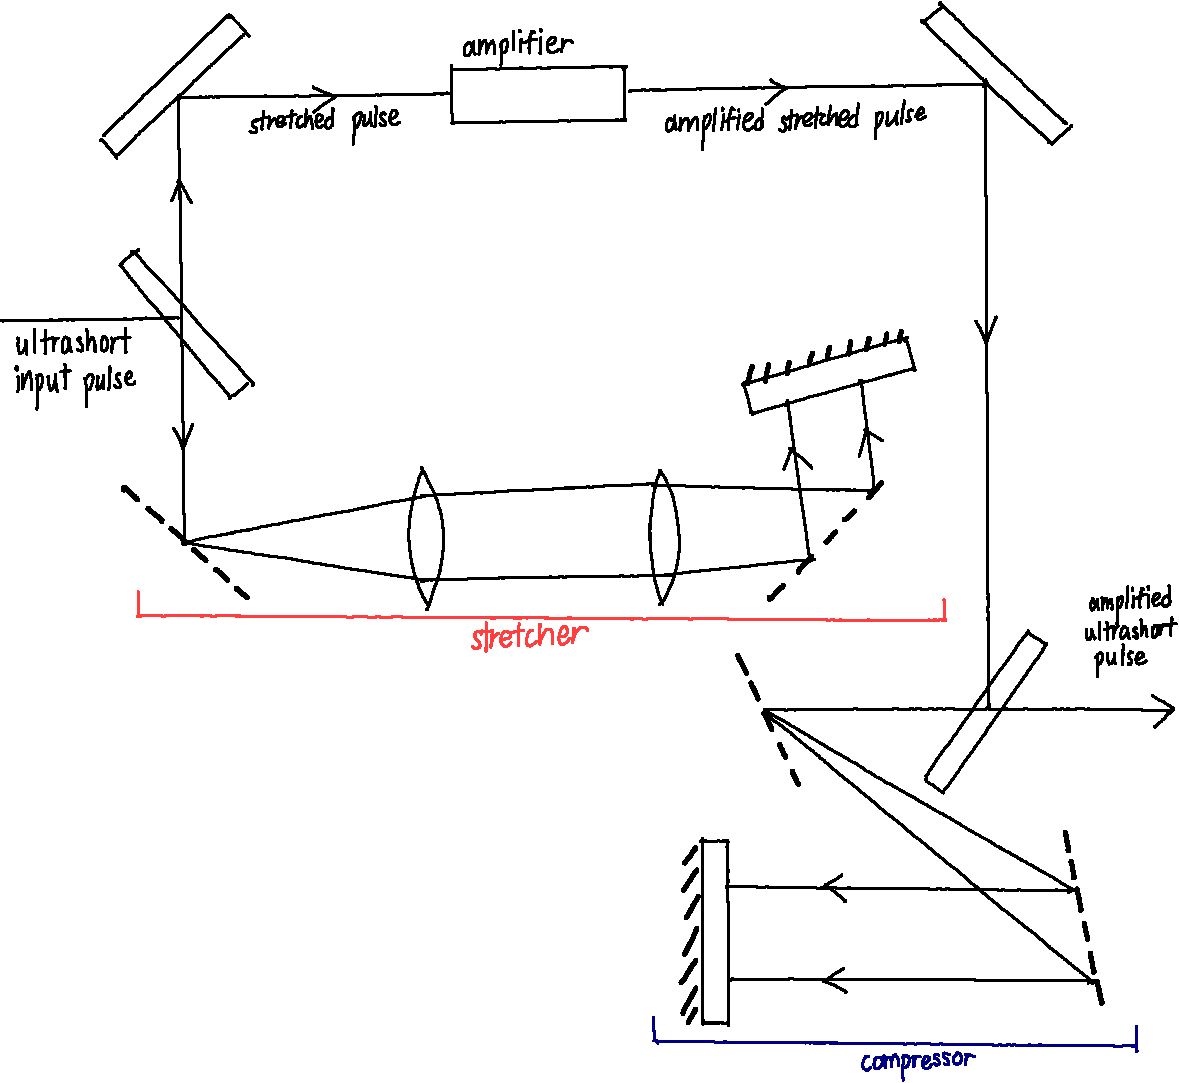
\includegraphics[width=.9\linewidth]{q1-cpa-setup}
	\end{figure}
	
	The stretcher applies positive GDD since most optical elements along the chain usually possess positive dispersion, hence avoiding accidental compression of the pulse.
	The stretched pulse is then amplified and passed to the compressor where negative GDD compresses the pulse back to the original length.
	
	\part From the given Gaussian pulse:
	\begin{align*}
		E(t) &= E_0 \exp\rbracket{-\Gamma t^2} \exp\rbracket{-i \omega_0 t} \\
		&= E_0 \exp\rbracket{-at^2} \exp\rbracket{-i(\omega_0 + bt)t}
	\end{align*}
	
	At HWHM $t=t_\diagfrac{1}{2}$, we have:
	\begin{gather*}
		\abs{E(t_\diagfrac{1}{2})}^2 = \frac{1}{2} \abs{E(0)}^2 \\
		\Rightarrow \exp\rbracket{-2at_\diagfrac{1}{2}} = \frac{1}{2} \\
		t_\diagfrac{1}{2} = \sbracket{\frac{\ln 2}{2a}}^{\frac{1}{2}}
	\end{gather*}
	
	Thus FWHM $\tau$ is:
	\begin{align*}
		\tau &= 2 t_\diagfrac{1}{2} \\
		&= 2 \sbracket{\frac{\ln 2}{2a}}^{\frac{1}{2}} \\
		&= \sbracket{\frac{2\ln 2}{a}}^{\frac{1}{2}}
	\end{align*}
	
	We also have phase gained by the pulse in time $t$: $\phi(t) = (\omega_0 + bt)t$.
	
	So we have instantaneous frequency:
	\begin{align*}
		\omega(t) &= \pderi{\phi}{t} \\
		&= \omega_0 + 2bt
	\end{align*}
	
	Recall that GDD is given by:
	\begin{align*}
		\phi^{(2)} &= \evalat{\pderi[2]{\phi}{\omega}}{\omega_0} \\
		&= \sbracket{
			\pdiff{\omega}\rbracket{
				\pderi{\phi}{t} \cdot \pderi{t}{\omega}
			}
		}_{\omega_0} \\
		&= \sbracket{
			\pdiff{\omega}\sbracket{
				(2b)^{-1} \, (\omega_0+2bt)
			}
		}_{\omega_0} \\
		&= \pdiff{t}\sbracket{
				(2b)^{-1} \, (\omega_0+2bt)
			}_{t=0}^{1} \cdot \evalat{\pderi{t}{\omega}}{t=0} \\
		&= \frac{1}{2b}
	\end{align*}
	
	Hence for positive chirp, $b > 0 \Rightarrow \textnormal{Im}(\Gamma) > 0$.
	
	\newpage
	\part Schematic of Michelson interferometer:
	\begin{figure}[H]
		\centering
		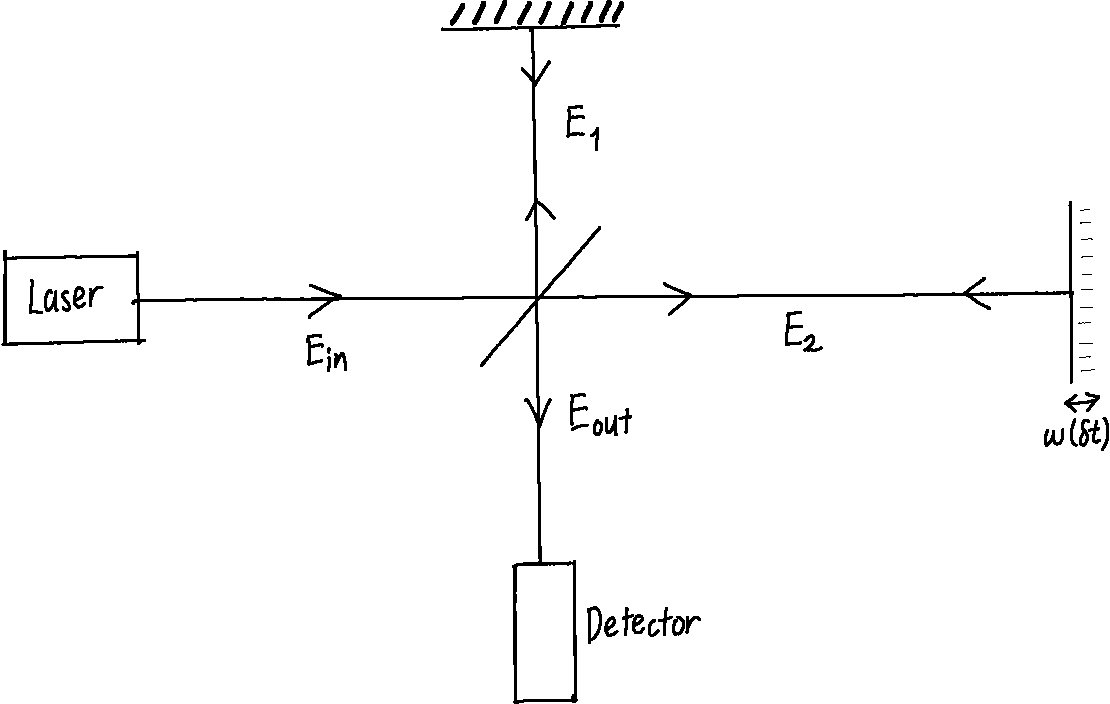
\includegraphics[width=.9\linewidth]{q1-michelson}
	\end{figure}
	
	After the beam splitter, we have $E_\textnormal{in} \rightarrow \frac{1}{2} E_\textnormal{in}$.
	
	Making the substitution $t \rightarrow t+\delta t$ then gives:
	\begin{align*}
		E_2 (t) &= \frac{E_0}{2} \, \mathrm{e}^{-\Gamma (t+\delta t)^2} \mathrm{e}^{-i\omega_0 (t+\delta t)} \\
		&= \frac{E_0}{2} \, \mathrm{e}^{-a (t+\delta t)^2} \mathrm{e}^{-ib(t+\delta t)^2} \mathrm{e}^{-i\omega_0 (t+\delta t)}
	\end{align*}
	
	Assuming $\delta t \ll t$, we then have $\mathrm{e}^{-a (t+\delta t)^2} \approx \mathrm{e}^{-at^2}$:
	\begin{align*}
		\Rightarrow E_2 (t) &= \frac{E_0}{2} \, \mathrm{e}^{-at^2} \mathrm{e}^{-i\omega_0 t} \mathrm{e}^{-ibt^2 - 2ibt(\delta t) - ib(\delta t)^2 - i\omega_0(\delta t)} \\
		&= \frac{E_0}{2} \, \mathrm{e}^{-at^2} \mathrm{e}^{-i\sbracket{\omega_0 + 2b(\delta t) + bt}t} \mathrm{e}^{-i\sbracket{b(\delta t)^2 + \omega_0 (\delta t)}}
	\end{align*}
	
	Hence the output E field is:
	\begin{align*}
		E_\textnormal{out}(t) &= E_1 + E_2 \\
		&= \frac{E_0}{2} \, \mathrm{e}^{-at^2} \sbracket{\mathrm{e}^{-i(\omega_0 + bt)t} + \mathrm{e}^{-i\sbracket{\omega_0 + 2b(\delta t) + bt}t} \mathrm{e}^{-i\sbracket{b(\delta t)^2 + \omega_0 (\delta t)}}} \\
		&= E_1 + E_2 \\
		&= \frac{E_0}{2} \, \mathrm{e}^{-at^2} \mathrm{e}^{-i(\omega_0 + bt)t} \sbracket{1 + \mathrm{e}^{-i\sbracket{2b(\delta t)t + b(\delta t)^2 + \omega_0 (\delta t)}}} \\
		&= \frac{E_0}{2} \, \mathrm{e}^{-at^2} \mathrm{e}^{-i(\omega_0 + bt)t} \mathrm{e}^{-\diagfrac{i}{2} \sbracket{2b(\delta t)t + b(\delta t)^2 + \omega_0 (\delta t)}} \cdot 2\cos\sbracket{\frac{[2b(\delta t)t + b(\delta t)^2 + \omega_0 (\delta t)}{2}} \\
		&= E_0 \mathrm{e}^{-at^2} \cos\sbracket{b (\delta t) \rbracket{t + \frac{\delta t}{2} + \frac{\omega_0}{2b}}} \mathrm{e}^{-i\bigl[\omega_0 t + \underbracket{\scriptstyle \rbracket{bt^2 + 2b(\delta t)t + b(\delta t)^2 + \omega_0(\delta t)}}_{\scriptstyle \psi(t) = b(t+\delta t)^2 + \omega_0 (\delta t)}\bigr]}
	\end{align*}
	
	The output intensity is then:
	\begin{align*}
		I_\textnormal{out} &= \abs{E_\textnormal{out}}^2 \\
		&= \abs{E_0}^2 \mathrm{e}^{-2at^2} \cos^2\sbracket{b (\delta t) \rbracket{t + \frac{\delta t}{2} + \frac{\omega_0}{2b}}}
	\end{align*}
	
	Sketch of $I_\textnormal{out}$ against $t$:
	\begin{figure}[H]
		\centering
		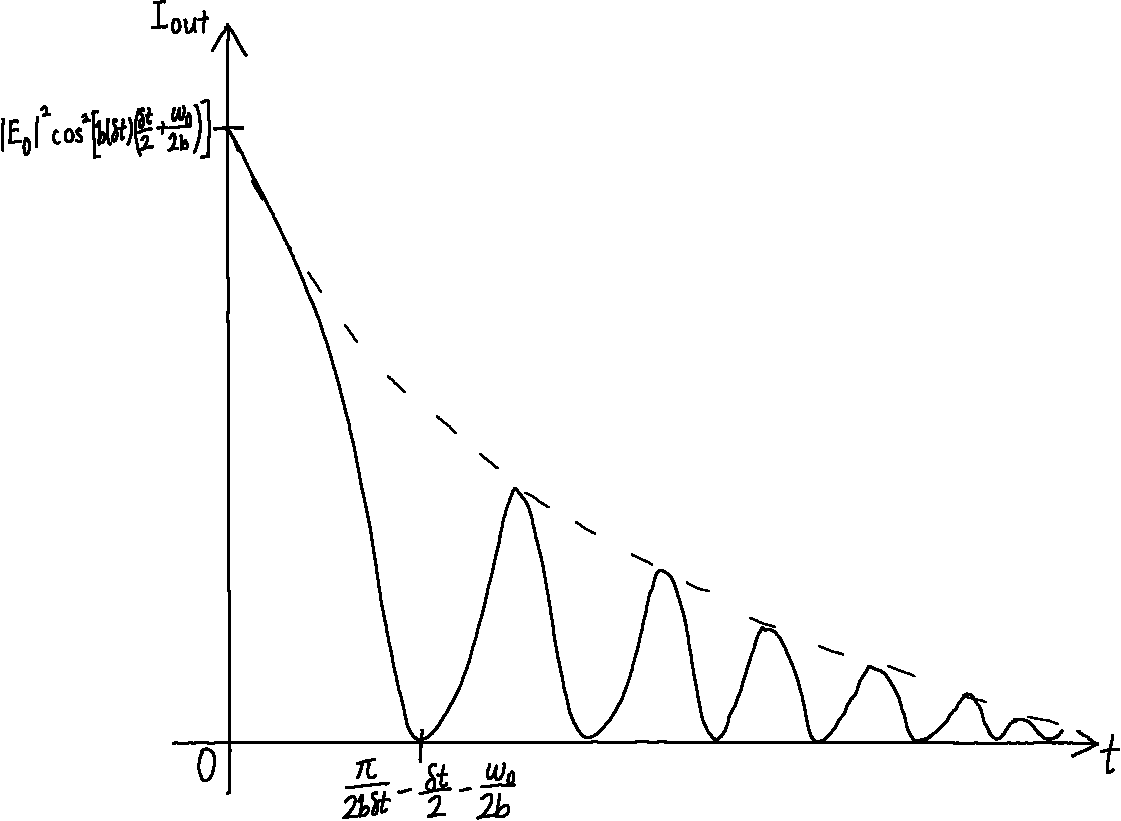
\includegraphics[width=.9\linewidth]{q1-iout}
	\end{figure}
	
	The intensity has a frequency of $b(\delta t)$.
	Hence the interval between adjacent peaks is:
	\begin{gather*}
		\rbracket{\Delta t} \cdot b(\delta t) = \pi \\
		\Rightarrow \Delta t = \frac{\pi}{b(\delta t)}
	\end{gather*}
	
	\part We know the frequency spectrum of $E_\textnormal{in}$ is given by the Fourier transform:
	\begin{align*}
		a(\omega) &= \frac{1}{\sqrt{2\pi}} \defint{-\infty}{\infty}{E_\textnormal{in}(t) \mathrm{e}^{i\omega t}}{t} \\
		&= \frac{1}{\sqrt{2\pi}} E_0 \mathrm{e}^{\rbracket{i\Omega / 2\Gamma^{1/2}}} \defint{-\infty}{\infty}{
			\mathrm{e}^{-\Gamma t^2 - i\Omega t - \rbracket{i\Omega / 2\Gamma^{1/2}}}
		}{t} \mtext{where $\Omega = \omega_0 - \omega$} \\
		&= \frac{1}{\sqrt{2\pi}} E_0 \mathrm{e}^{-\Omega^2 / 4\Gamma} \underbracket{\defint{-\infty}{\infty}{
			\mathrm{e}^{-\rbracket{\Gamma^{1/2} t + i\Omega/2\Gamma^{1/2}}^2}
		}{t}}_{
			\displaystyle \defint{-\infty}{\infty}{\mathrm{e}^{\Gamma \rbracket{t + i\Omega/2\Gamma}^2}}{t} = \sqrt{\frac{\pi}{\Gamma}}
		} \\
		&= \frac{1}{\sqrt{2\pi}} E_0 \sqrt{\frac{\pi}{\Gamma}} \, \mathrm{e}^{-\Omega^2/4\Gamma}
	\end{align*}
	
	Thus the power spectrum is:
	\begin{align*}
		P(\omega) &= \abs{a(\omega)}^2 \\
		&= \frac{1}{2\pi} \abs{E_0}^2 \cdot \frac{\pi}{|\Gamma|} \abs{\mathrm{e}^{-(\omega_0 - \omega)^2 / 4\Gamma}}^2
	\end{align*}
	
	Now for a Michelson interferometer, we have total average intensity\footnote{Point of confusion: $I(t)$ or $I(\delta t)$? It turns out that when we are integrating $P(\omega)$ what we are doing is to find the average intensity over a long time (see page 223 of Brooker)}:
	
	\begin{equation}
		I(\delta t) = \defint{0}{\infty}{P(\omega) \cdot \frac{1 + \cos\rbracket{\omega(\delta t)}}{2}}{\omega}
		\label{eqn:q1-total-average-intensity}
	\end{equation}
	
	Now we have:
	\begin{align*}
		\mathrm{e}^{-(\omega_0 - \omega)^2 / 4\Gamma} &= \mathrm{e}^{-(\omega_0 - \omega)^2 / 4 \cdot a-ib/a^2+b^2} \\
		&= \mathrm{e}^{-(\omega_0 - \omega)^2 / 4(a^2 + b^2) \cdot a} \mathrm{e}^{+i (\omega_0 - \omega)^2 / 4(a^2 + b^2) \cdot b} \\
		\Rightarrow \abs{\mathrm{e}^{(\omega_0 - \omega)^2 / 4\Gamma}}^2 &= \mathrm{e}^{- a(\omega_0 - \omega)^2 / 2(a^2 + b^2)}
	\end{align*}
	
	\eqref{eqn:q1-total-average-intensity} then becomes:
	\begin{align*}
		I(\delta t) &= \defint{0}{\infty}{
			\frac{\abs{E_0}^2 \pi}{2\pi \abs{\Gamma}} \mathrm{e}^{-a(\omega_0 - \omega)^2 / 2(a^2+b^2)} \cdot \frac{1 + \cos\rbracket{\omega (\delta t)}}{2}
		}{\omega} \\
		&\propto \defint{-\infty}{\infty}{
			\mathrm{e}^{-a(\omega_0 - \omega)^2 / 2(a^2+b^2)} \sbracket{1 + \cos\rbracket{\omega (\delta t)}}
		}{\omega} \mtext{since the integrand is even in $\omega$} \\
		&\propto \textnormal{Re} \sbracket{
			\defint{-\infty}{\infty}{
				\mathrm{e}^{-a(\omega_0 - \omega)^2 / 2(a^2+b^2)} \mathrm{e}^{-i\omega(\delta t)}
				}{\omega}}
			\mtext{\parbox[t]{16em}{since the first term is constant and the second term may be written as $\cos\rbracket{\omega(\delta t)} + i\sin\rbracket{\omega(\delta t)}$ with the imaginary integrand vanishing due to it being odd}} \\
		&= \textnormal{Re} \sbracket{\defint{-\infty}{\infty}{\mathrm{e}^{-A\omega^2 - \rbracket{i(\delta t)-2A\omega_0}\omega - A\omega_0^2}}{\omega}} \mtext{where $A = \dfrac{a}{2(a^2+b^2)}$} \\
		&= \textnormal{Re} \sbracket{
			\defint{-\infty}{\infty}{
				\mathrm{e}^{-A\omega^2 - \rbracket{i(\delta t)-2A\omega_0}\omega - \rbracket{\frac{i(\delta t) - 2A\omega_0}{2A^{1/2}}}^2}
				\mathrm{e}^{\rbracket{
						\frac{i(\delta t) - 2A\omega_0}{2A^{1/2}}
					}^2 - A\omega_0^2}
			}{\omega}
		} \\
		&= \textnormal{Re} \sbracket{
				\mathrm{e}^{-(\delta t)^2/4A} \mathrm{e}^{-i\omega_0 (\delta t)} 
				\underbracket{
					\defint{-\infty}{\infty}{
						\mathrm{e}^{-A(\omega + \ldots)^2}
					}{\omega}}
				_{\sqrt{\frac{\pi}{A}}}
			} \\
		&= \sqrt{\frac{\pi}{A}} \mathrm{e}^{-(\delta t)^2/4A} \cos\rbracket{\omega_0 (\delta t)}
	\end{align*}
	
	So $I(\delta t)$ has frequency $\omega_0 \rightarrow \omega_0+2bt$ to account for the shifting of mean sample frequency due to chirping.
	
	Thus adjacent peaks would have an interval of:
	\begin{align*}
		2b(\Delta t)(\delta t) &= 2\pi \\
		\Delta t &= \frac{\pi}{b(\delta t)}
	\end{align*}
	which matches the result from part c.
	
	As $\delta t$ increases, the average intensity $I(\delta t)$ rapidly drops and approaches $0$ due to the exponential prefactor, suggesting that there is a limitation in how far a measurement in $\delta t$ can go.
\end{parts}